\section{Definição}

\begin{frame}[fragile]{Listas circulares}

    \begin{itemize}
        \item Uma lista circular é uma lista onde o membro  \code{c}{next} do último elemento
            aponta para o primeiro elemento, e o campo \code{c}{prev} do primeiro elemento
            aponta para o último elemento, quando for o caso

        \item A lista forma um caminho cíclico entre seus elementos, de modo que a identificação
            do primeiro ou do último elemento é, de fato, relativa

        \item Uma travessia deve marcar um ponto de partida e progredir até que atinja este
            ponto novamente, encerrando assim a travessia

        \item Em geral, as listas circulares são implementadas como listas encadeadas

        \item As operações de inserção e remoção em uma posição conhecida tem complexidade
            constante
    \end{itemize}

\end{frame}

\begin{frame}[fragile]{Visualização de uma lista circular}

    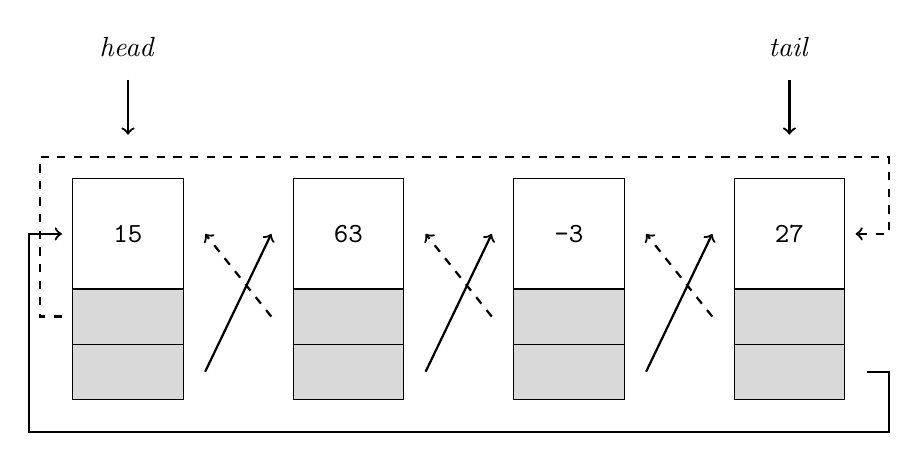
\begin{tikzpicture}[scale=1.4]
        \node[anchor=center] at (0.5, 3.2) {\textit{head}};
        \draw[->,thick] (0.5, 2.9) -- (0.5, 2.4);

        \node[anchor=center] at (6.5, 3.2) {\textit{tail}};
        \draw[->,thick] (6.5, 2.9) -- (6.5, 2.4);

        \draw[->,thick] (7.2, 0.25) -- (7.4, 0.25) -- (7.4, -0.3) -- (-0.4, -0.3) -- (-0.4, 1.5)
            -- (-0.1, 1.5);
        \draw[->,thick,dashed] (-0.1, 0.75) -- (-0.3, 0.75) -- (-0.3, 2.2) -- (7.4, 2.2) -- (7.4, 1.5) -- (7.1, 1.5);

        \draw[fill=white] (0,1) rectangle (1,2);
        \draw[fill=gray!30] (0,0.5) rectangle (1,1);
        \draw[fill=gray!30] (0,0) rectangle (1,0.5);
        \node at (0.5,1.5) {\texttt{15}};

        \draw[->,thick] (1.2, 0.25) -- (1.8, 1.5);
        \draw[->,thick,dashed] (1.8, 0.75) -- (1.2, 1.5);

        \draw[fill=white] (2,1) rectangle (3,2);
        \draw[fill=gray!30] (2,0) rectangle (3,0.5);
        \draw[fill=gray!30] (2,0.5) rectangle (3,1);
        \node at (2.5,1.5) {\texttt{63}};

        \draw[->,thick] (3.2, 0.25) -- (3.8, 1.5);
        \draw[->,thick,dashed] (3.8, 0.75) -- (3.2, 1.5);

        \draw[fill=white] (4,1) rectangle (5,2);
        \draw[fill=gray!30] (4,0) rectangle (5,0.5);
        \draw[fill=gray!30] (4,0.5) rectangle (5,1);
        \node at (4.5,1.5) {\texttt{-3}};

        \draw[->,thick] (5.2, 0.25) -- (5.8, 1.5);
        \draw[->,thick,dashed] (5.8, 0.75) -- (5.2, 1.5);

        \draw[fill=white] (6,1) rectangle (7,2);
        \draw[fill=gray!30] (6,0) rectangle (7,0.5);
        \draw[fill=gray!30] (6,0.5) rectangle (7,1);
        \node at (6.5,1.5) {\texttt{27}};

    \end{tikzpicture}

\end{frame}

